\usepackage{xcolor}
\usepackage{afterpage}
\usepackage{pifont,mdframed}
\usepackage[bottom]{footmisc}

\makeatletter
\gdef\this@inputfilename{input}
\gdef\this@outputfilename{output}
\makeatother

\newcommand{\funcitem}[2]{\item[$\blacksquare$] \textbf{\large \textsf{Funzione} \texttt{#1}} \vspace{-0.3cm} \begin{center}\begin{tabularx}{\textwidth}{|c|X|} \hline #2 \hline \end{tabularx}\end{center}}

Facendo pulizia in soffitta Fabio ha ritrovato diversi quadri, alcuni del tutto privi di valori e altri invece potenzialmente interessanti (tra cui diverse copie di alcuni dipinti di Leonardo da Vinci). Per racimolare qualche soldo, ha intenzione di venderli: ha pertanto portato a valutare gli $N$ quadri da un esperto che ha attribuito a ciascuno un valore $V_i$ approssimativo.

Per far sì che tutti i quadri di minor valore non restino invenduti, continunando a ingombrare la soffitta, Fabio è intenzionato a organizzare una lotteria con una regola particolare: le opere saranno disposte in fila e l'acquirente, dopo aver pagato un ``biglietto di ingresso'', potrà scegliere a propria discrezione un ``blocco'' consecutivo di $B$ opere (non di più né di meno). 

\begin{figure}[H]
  \begin{center}
        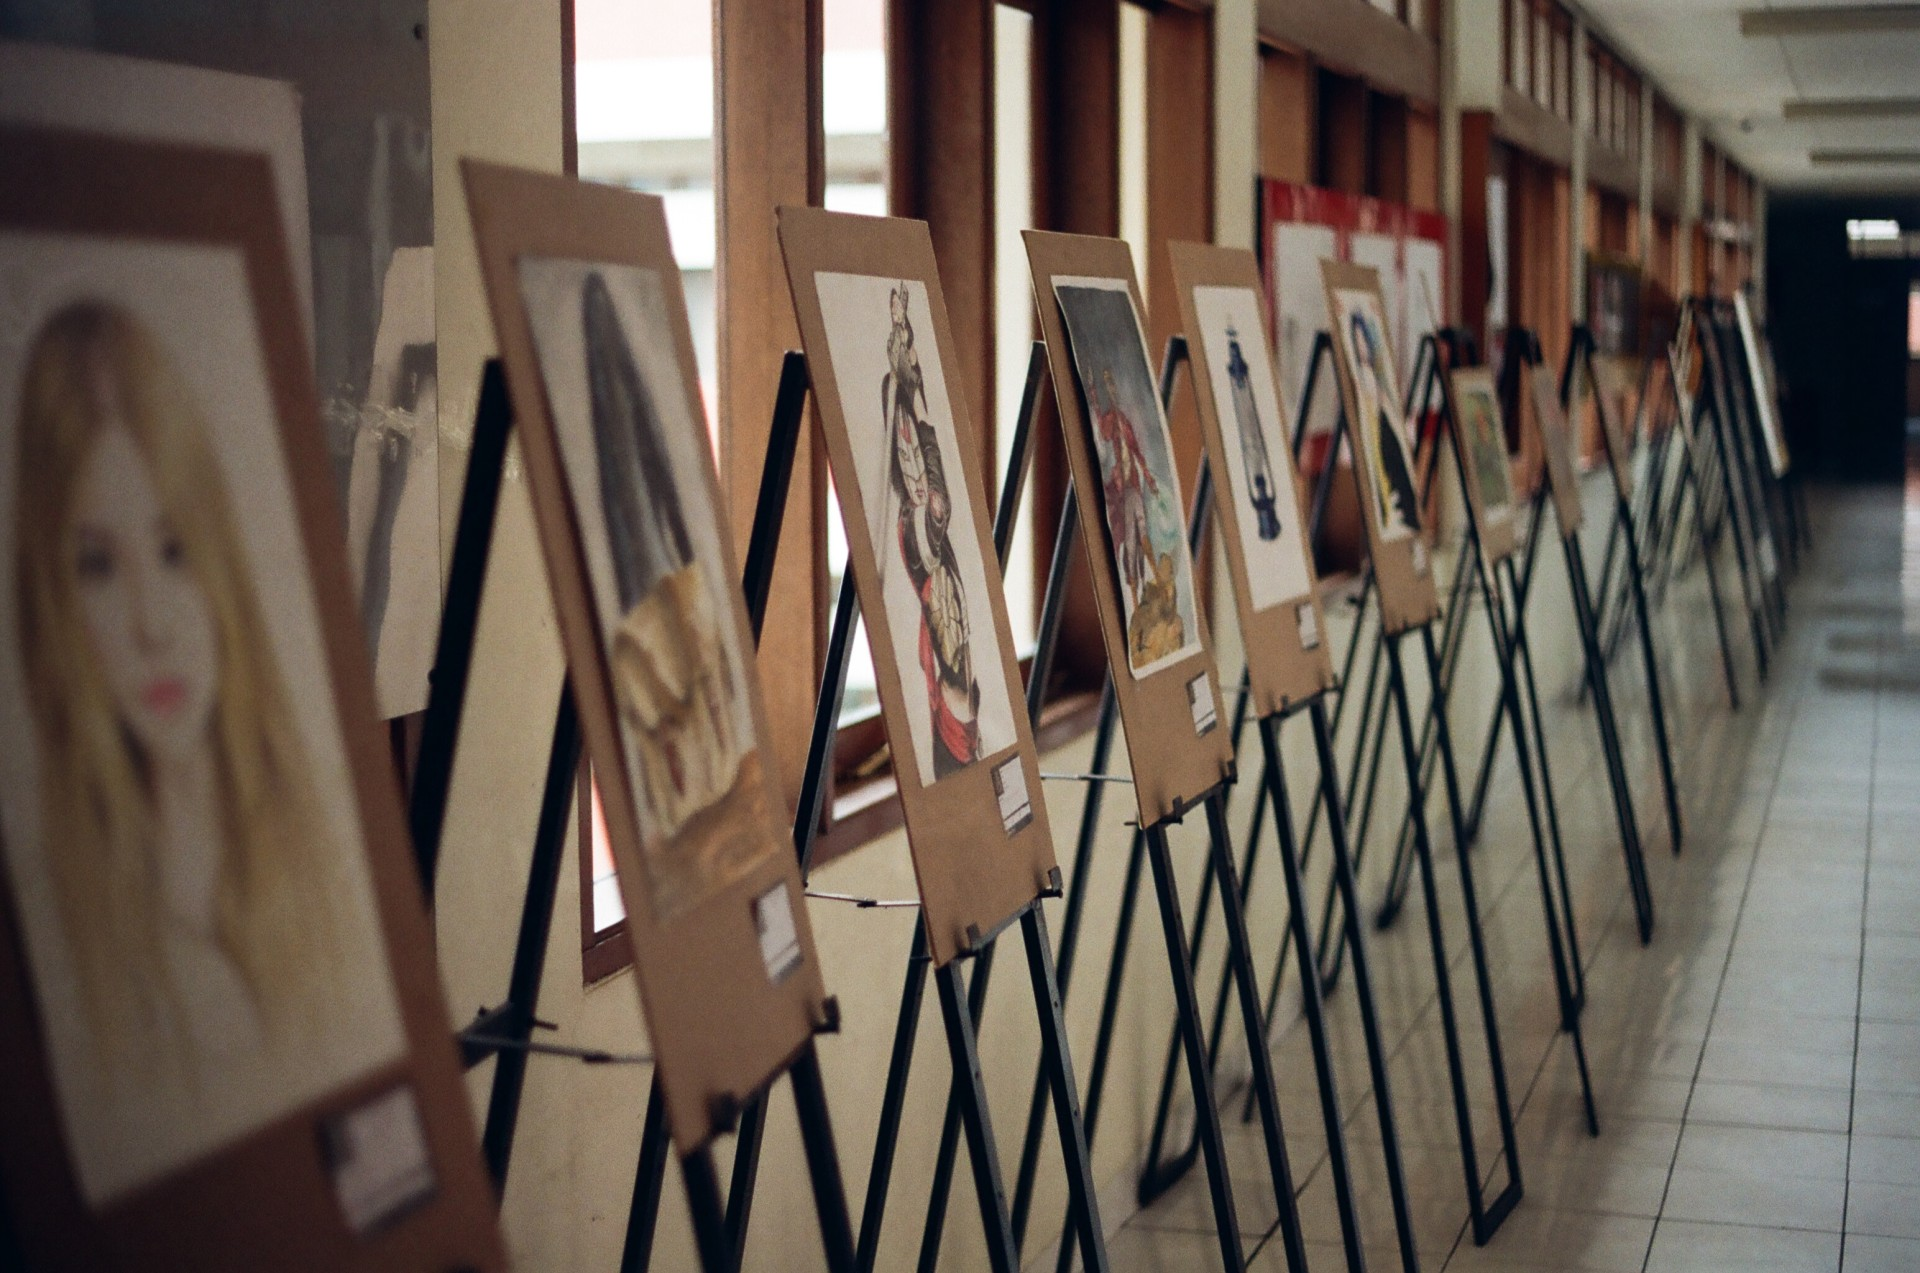
\includegraphics[width=0.7\linewidth]{quadri.jpg}
    \caption{Alcuni dei quadri esposti (\href{https://unsplash.com/photos/9JEYfqLj-H0}{foto di Muhammad Raufan Yusup}).}
  \end{center}
\end{figure}

Fabio non vuole che la somma dei valori delle opere che un acquirente può portarsi a casa sia maggiore di un certo massimale $M$, altrimenti ci starebbe perdendo troppo. D'altro canto, pur rispettando questo principio, vorrebbe rendere $B$ (il numero di quadri che ci si porta a casa comprando il biglietto d'ingresso) più alto possibile. Aiutalo a capire qual è il valore massimo di $B$ per rendere il più appetibile possibile la lotteria!

\Implementation

Dovrai sottoporre un unico file con estensione \texttt{.cpp} o \texttt{.c}.

\begin{warning}
Tra gli allegati a questo task troverai un template (\texttt{quadri.cpp} e \texttt{quadri.c}) con un esempio di implementazione.
\end{warning}

\pagebreak

Dovrai implementare la seguente funzione:

\begin{itemize}[nolistsep]
    \funcitem{quadri}{
        C/C++  & \verb|int quadri(int N, long long M, int V[]);|\\
    }

    \begin{itemize}[nolistsep]
        \item L'intero $N$ rappresenta il numero dei quadri.
        \item L'intero $M$ rappresenta il massimale da non superare.
        \item L'array \texttt{V}, indicizzato da $0$ a $N-1$, contiene alla posizione $i$ il valore dell'$i$-esimo quadro nella fila.
        \item La funzione dovrà restituire il valore massimo per $B$ come descritto nel testo.

    \end{itemize}
\end{itemize}

Il grader chiamerà la funzione \texttt{quadri} e ne stamperà il valore restituito sul file di output.

% % % % % % % % % % % % % % % % % % % % % % % % % % % % % % % % % % % % % % % % % % %
% % % % % % % % % % % % % % % % % % % % % % % % % % % % % % % % % % % % % % % % % % %


\Grader
Allegata a questo problema è presente una versione semplificata del grader usato durante la correzione, che potete usare per testare le vostre soluzioni in locale. Il grader di esempio legge i dati da \texttt{stdin}, chiama la funzione che dovete implementare e scrive su \texttt{stdout}, secondo il seguente formato.

Il file di input è composto da due righe, contententi:

\begin{itemize}[nolistsep,itemsep=2mm]
    \item Riga $1$: gli interi $N$ e $M$, separati da uno spazio.
    \item Riga $2$: $N$ interi \texttt{V[$i$]} per $i = 0,\ldots, N-1$.
\end{itemize}

Il file di output è composto da un'unica riga, contenente:
\begin{itemize}[nolistsep,itemsep=2mm]
    \item Riga $1$: il valore restituito dalla funzione \texttt{quadri}.
\end{itemize}

% % % % % % % % % % % % % % % % % % % % % % % % % % % % % % % % % % % % % % % % % % %
% % % % % % % % % % % % % % % % % % % % % % % % % % % % % % % % % % % % % % % % % % %

\Constraints

\begin{itemize}[nolistsep, itemsep=2mm]
\item $1 \le N \le 200\,000$.
\item $1 \le M \le 10^{12}$.
\item $1 \le V_i \le 10^{6}$ per ogni $i = 0 \ldots N-1$.
\item Nella scelta del blocco di $B$ quadri, l'acquirente \textbf{non} può scegliere un blocco agli estremi della fila in modo da prenderne meno di $B$.
\end{itemize}

\Scoring
Il tuo programma verrà testato su diversi test case raggruppati in subtask.
Per ottenere il punteggio relativo ad un subtask, è necessario risolvere
correttamente tutti i test relativi ad esso.
\begin{itemize}[nolistsep,itemsep=2mm]
\item \textbf{\makebox[2cm][l]{Subtask 1} [\phantom{0}0 punti]}: Casi d'esempio.
\item \textbf{\makebox[2cm][l]{Subtask 2} [15 punti]}: $M < V_i$ per ogni $i = 0,\ldots,N-1$ oppure $M > V_0 + V_1 + \ldots + V_{N-1}$.
\item \textbf{\makebox[2cm][l]{Subtask 3} [20 punti]}: $N \le 500$.
\item \textbf{\makebox[2cm][l]{Subtask 4} [25 punti]}: $N \le 5\,000$.
\item \textbf{\makebox[2cm][l]{Subtask 5} [40 punti]}: Nessuna limitazione specifica.
\end{itemize}

\pagebreak

\Examples
\begin{example}
\exmpfile{quadri.input0.txt}{quadri.output0.txt}%
\exmpfile{quadri.input1.txt}{quadri.output1.txt}%
\end{example}

\Explanation

Nel \textbf{primo caso di esempio} è possibile impostare $B=2$: l'acquirente potrebbe scegliere i quadri di valore $1+2=3$, $2+3=5$ oppure $3+4=7$ senza superare mai il massimale $M=8$. Non sarebbe stato possibile scegliere $B=3$ perché in quel caso l'acquirente avrebbe potuto il scegliere il blocco di valore $2+3+4=9$, superando il massimale.

Nel \textbf{secondo caso di esempio} anche scegliere $B=1$ consentirebbe all'acquirente di superare il massimale qualunque scelta egli faccia (ad eccezione del secondo quadro). La risposta corretta è quindi $B=0$.
